%%%%%%%%%%%%%%%%%%%%%%%%%%%%%%%%%%%%%%%%%%%%%%%%%%%%%%%%
% Este é um documento que servirá de modelo para
% os relatórios feitos na disciplina Laboratório de Circuitos Lógicos
% 2020-2
%%%%%%%%%%%%%%%%%%%%%%%%%%%%%%%%%%%%%%%%%%%%%%%%%%%%%%%%%

%%%%%%%%%%%%%%%%%%%%%%%%%%%%%%%%%%%%%%%%%%%%%%%%%%%%%%%%%
% Use os diferentes diretórios para colocar os relatórios de cada experimento, deste modo vc consegue manter um histórico e todo material organizado em apenas um local.
% Lembre-se de mudar o Main Document no Menu!!!

\documentclass[12pt]{article}

\usepackage{sbc-template}
\usepackage[brazil,american]{babel}
\usepackage[utf8]{inputenc}

\usepackage{graphicx}
\usepackage{url}
\usepackage{float}
\usepackage{listings}
\usepackage{color}
\usepackage{todonotes}
\usepackage{algorithmic}
\usepackage{algorithm}
\usepackage{hyperref}
\usepackage{amsmath}
\usepackage{graphicx}
\usepackage{array}
\usepackage[shortlabels]{enumitem}

\sloppy


\title{Experimento 4\\
Circuitos Combinacionais: Comparador de Palavras}

\author{Matheus Cardoso de Souza, 202033507\\
        Ualiton Ventura da Silva, 202033580\\
        Grupo G42
}

%%%% LEMBRE-SE DE MUDAR O GRUPO NA LINHA ABAIXO!!!!! %%%%%%
\address{Dep. Ciência da Computação -- Universidade de Brasília (UnB)\\
  CIC0231 - Laboratório de Circuitos Lógicos
  \email{matheus-cardoso.mc@aluno.unb.br, 202033580@aluno.unb.br}
}

\begin{document}
\maketitle

\selectlanguage{american}
 \begin{abstract}
   TODO
 \end{abstract}
\selectlanguage{brazil}

 \begin{resumo}
   TODO
 \end{resumo}


\section{Introdução}
\label{sec:Introducao}

% Escreva com suas palavras o que vai ser trabalhado no experimento. Aqui temos um exemplo de como citar a bibliografia consultada \cite{boulic:91} \cite{smith:99}.

TODO

\subsection{Objetivos}
\label{sec:Objetivos}

TODO

\subsection{Materiais}
\label{sec:Materiais}
Em função da natureza do ensino a distância, os presentes experimentos não foram
realizados usando-se materiais e equipamentos físicos, mas sim emulados por meio
do simulador online \href{https://www.tinkercad.com/}{Tinkercad}, e também do
\href{https://www.digitalelectronicsdeeds.com/deeds.html}{Deeds}.

A seguir estão enumerados os materiais simulados:
\begin{itemize}
    \item Painel Digital
    \item \textit{Protoboard}
    \item Fios
    \item Seletores de estado lógico
    \item LEDs
    \item Resistores
    \item Multímetros
    \item Portas Lógicas \textbf{NAND}
\end{itemize}

\section{Procedimentos}
\label{sec:Procedimentos}

Passaremos a apresentar os experimentos requeridos.

\subsection{Atraso de Propagação em portas lógicas}\label{sec:atraso_de_propagação}

\begin{enumerate}[A)]
\item \textbf{Equações Lógicas de L0 e L1}
\end{enumerate}

Começaremos com a equação lógica \textbf{L1}, pois \textbf{L0} depende dessa. Temos que, como
o número de portas \textbf{NOT} que ligam o sinal de clock \textbf{A} à
\textbf{L1} é \emph{ímpar}, a saída terá o sinal de \textbf{A} negado. Sendo
assim, concluímos que a equação para \textbf{L1} será:

\begin{equation}
L1 = \overline{A}
\end{equation}

Agora, considerando a saída \textbf{L0}, podemos verificar que existe uma porta
\textbf{AND} tomando o resultado de \textbf{A} e \textbf{L1}. Portanto, a equação de \textbf{L0} será:

\begin{equation}
L0 = A \cdot L1\label{eq:L0}
\end{equation}

Dessa forma, podemos expressar ambos \textbf{L0} e \textbf{L1} por meio de uma
tabela verdade, em função de \textbf{A}.

\begin{table}[H]
    \centering
    \caption{\textbf{L0} e \textbf{L1} em função de \textbf{A}}
    \begin{tabular}{|c|c|c|}\hline
        \multicolumn{1}{|c|}{Entrada} & \multicolumn{2}{|c|}{Saídas} \\\hline
        \textbf{A} & \textbf{L0} & \textbf{L1} \\\hline
        0 & 0 & 1 \\\hline
        1 & 0 & 0 \\\hline
    \end{tabular}\label{tab:atraso_de_propagação:L0_L1}
\end{table}

\begin{enumerate}[B)]
\item \textbf{Comportamento de L0 e L1}
\end{enumerate}

Utilizando a ferramenta
\href{https://www.digitalelectronicsdeeds.com/deeds.html}{Deeds} para a
simulação do circuito lógico, podemos observar que as saídas de \textbf{L0} e
\textbf{L1} são exatamente as esperadas quando leva-se em conta a tabela verdade
\ref{tab:atraso_de_propagação:L0_L1} apresentada acima.

Como representado nas figuras a seguir, o output de \textbf{L0} é \emph{sempre}
igual a $0$, e o output de \textbf{L1} é \emph{sempre} o oposto de \textbf{A},
assim como esperado.

\begin{figure}[H]
    \centering
    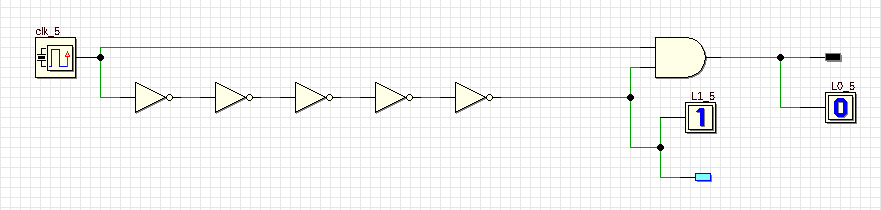
\includegraphics[width=.9\textwidth]{Exp04/exp4_2.0_b_clk_up.png}
    \caption{Clock Up}\label{fig:exp4_2.0_b_clk_up.png}
\end{figure}

\begin{figure}[H]
    \centering
    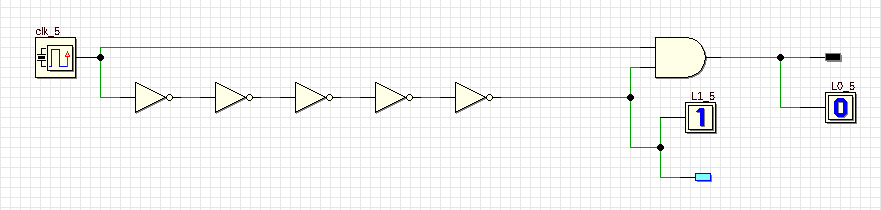
\includegraphics[width=.9\textwidth]{Exp04/exp4_2.0_b_clk_down.png}
    \caption{Clock Down}\label{fig:exp4_2.0_b_clk_down.png}
\end{figure}

\begin{enumerate}[C)]
\item \textbf{Formas de onda para L0 e L1}
\end{enumerate}

Utilizando a ferramenta \emph{Timing Diagram Simulation} podemos gerar as
formas de onda para \textbf{L0} e \textbf{L1}. A seguir reproduzimos as mesmas.

\begin{figure}[H]
    \centering
    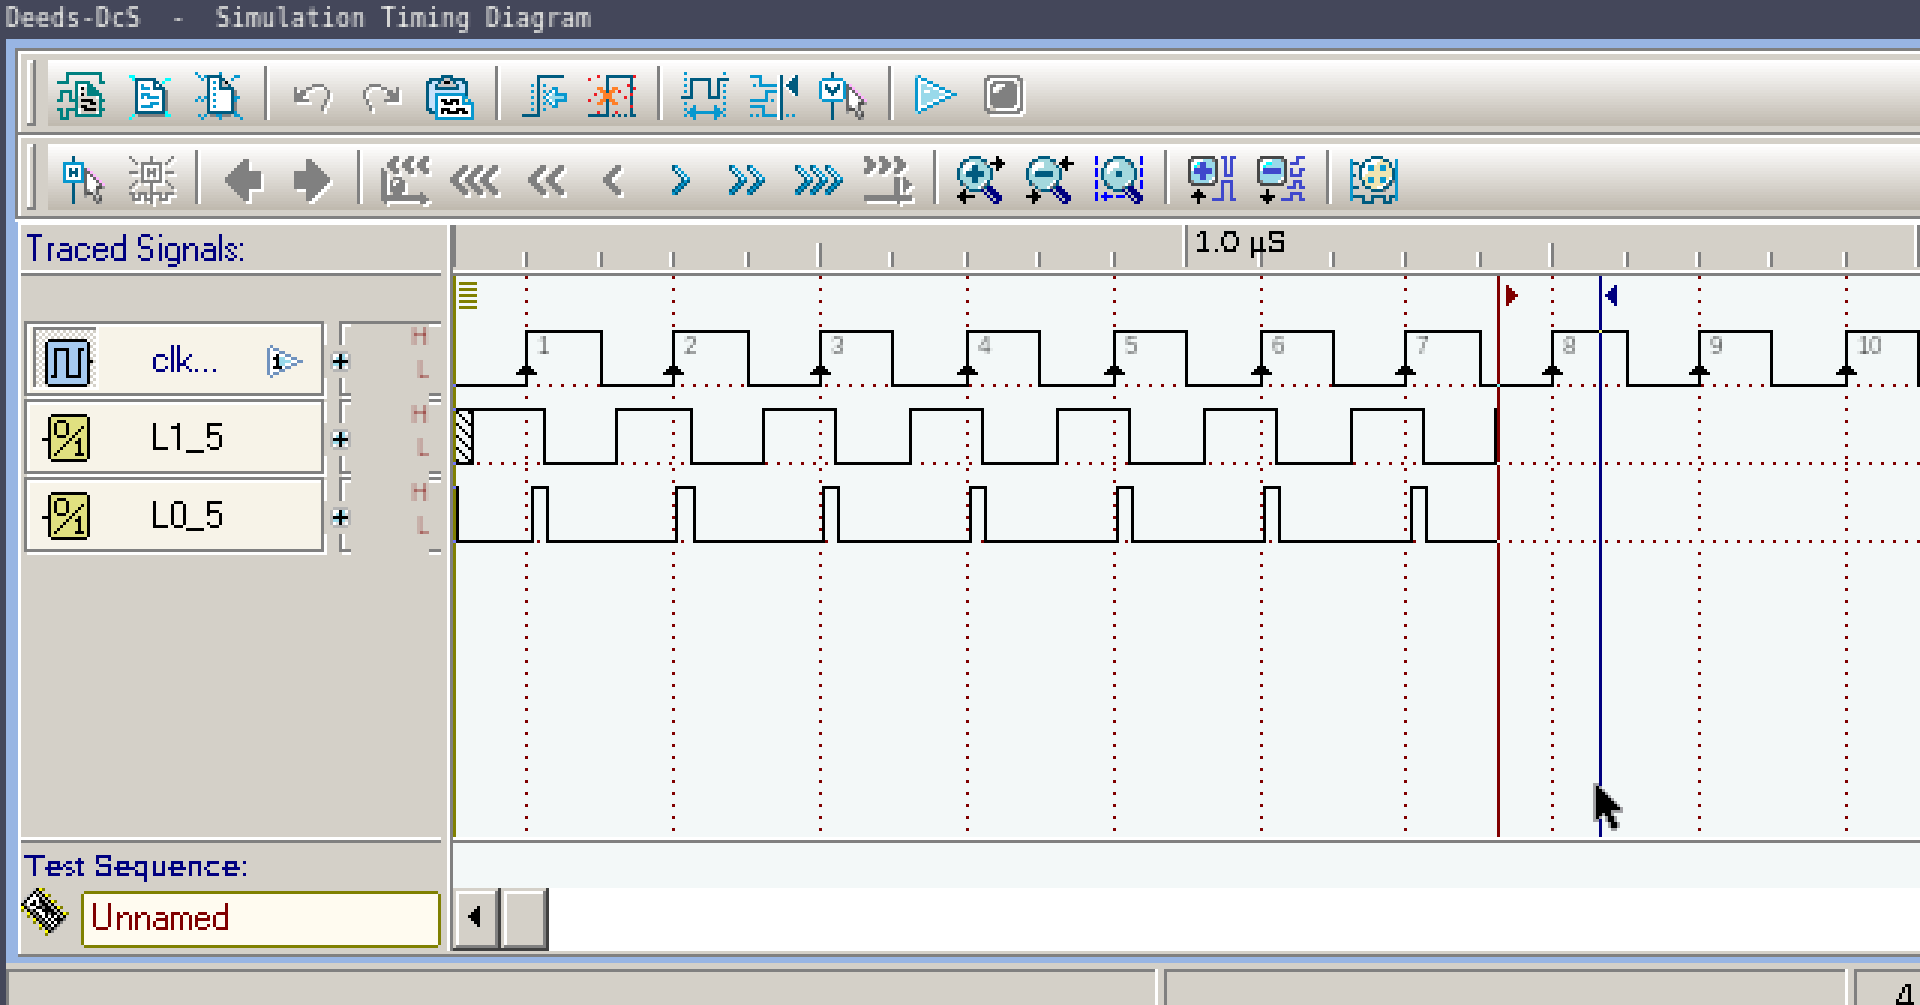
\includegraphics[width=1\textwidth]{Exp04/exp4_2.0_c_clk_wave.png}
    \caption{Clock Up}\label{fig:exp4_2.0_c_clk_wave.png}
\end{figure}

Como pode-se observar, a saída \textbf{L0} possui um pequeno pulso quando o
clock varia. Podemos explicar esse comportamento levando em consideração o delay
que as portas lógicas possuem. Como a porta lógica \textbf{L0} possui como um de
seus inputs a porta \textbf{L1}, que por sua vez tem um delay de $5$ portas
\textbf{NOT}, a porta \textbf{L0} soma um delay de $5$ portas \textbf{NOT} e $1$
porta \textbf{AND}. Dessa forma, a soma total resulta em um delay de $21ns$,
como pode-se ver na imagem a seguir.

\begin{figure}[H]
    \centering
    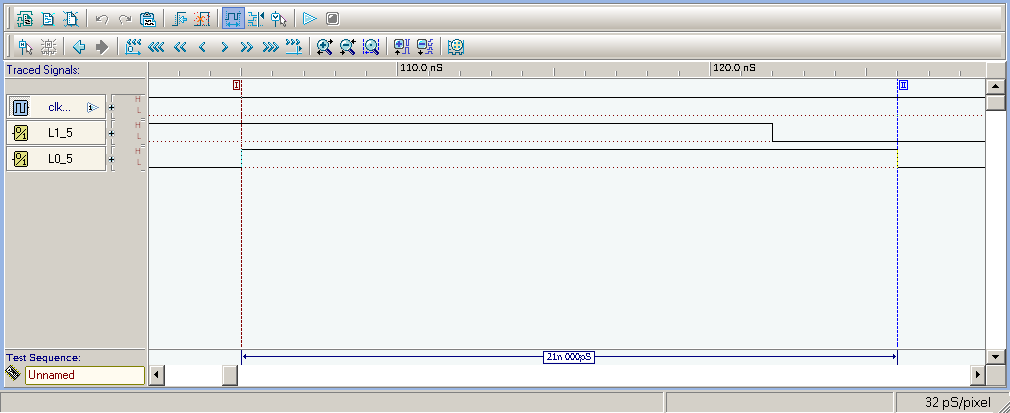
\includegraphics[width=.9\textwidth]{Exp04/exp4_2.0_c_clk_wave_lenght.png}
    \caption{Comprimento do pulso em \textbf{L0}}\label{fig:exp4_2.0_c_clk_wave_lenght.png}
\end{figure}

\begin{enumerate}[D)]
\item \textbf{Pulsos em L0 quando A retorna ao nível 0}
\end{enumerate}

De forma sucinta, podemos afirmar que, para o circuito específico deste
exercício, contendo $5$ portas \textbf{NOT} e $1$ porta \textbf{AND}, não existe
pulso em \textbf{L0} quando \textbf{A} retorna ao nível $0$.

Para justificar tal afirmação precisamos considerar qual a função lógica
responsável por produzir o output em \textbf{L0}. Lembrando da equação
\ref{eq:L0}, vemos que a única forma de termos um pulso em \textbf{L0} seria se
\textbf{L1} fosse $1$ no momento que \textbf{A} retorna ao nível $0$. Podemos
afirmar isso pois consideramos o delay da porta \textbf{AND} responsável pelo
output de \textbf{L0}. Logo, o pulso seria consideravelmente menor que o
existente na passagem de nível lógico \textbf{A} $= \, 0$ para \textbf{A}
$= \, 1$, mas seria possível existir. Cabe ressaltar, entretanto, que o pulso em
\textbf{L0} \emph{não} aconteceria na montagem de apenas $5$ portas
\textbf{NOT}, pois o delay não seria sufucientemente grande. Na imagem a seguir
apresentamos uma possível configuração de circuito lógico, contendo um número
\emph{ímpar} de portas \textbf{NOT}, que tem de fato um pulso em \textbf{L0}
quando \textbf{A} está retornando ao nível $0$.

\begin{figure}[H]
    \centering
    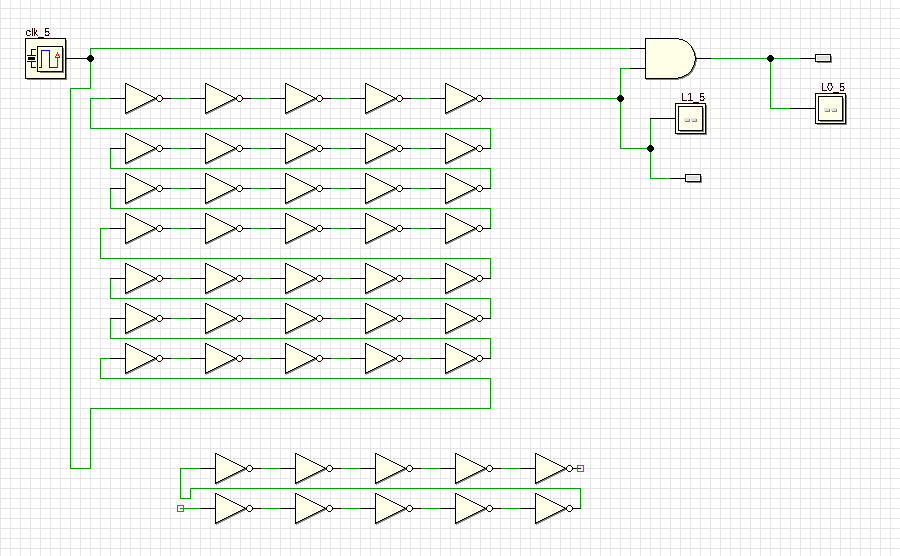
\includegraphics[width=.9\textwidth]{Exp04/exp4_2.0_d_clk_circuito_ao_voltar_para_zero.png}
    \caption{Circuito que apresenta pulso quando \textbf{A} retorna ao nível 0}\label{fig:exp4_2.0_d_clk_circuito_ao_voltar_para_zero.png}
\end{figure}

\begin{figure}[H]
    \centering
    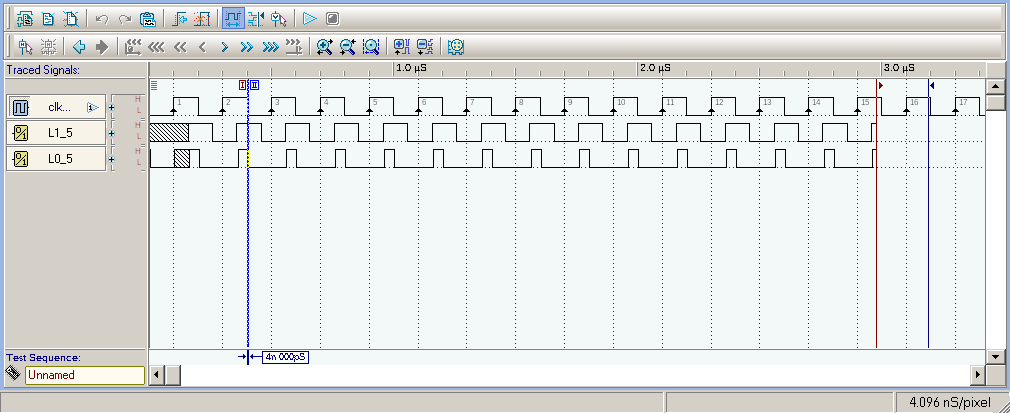
\includegraphics[width=.9\textwidth]{Exp04/exp4_2.0_d_clk_wave_ao_voltar_para_zero.png}
    \caption{Formato de onda desse circuito}\label{fig:exp4_2.0_d_clk_wave_ao_voltar_para_zero.png}
\end{figure}

\begin{figure}[H]
    \centering
    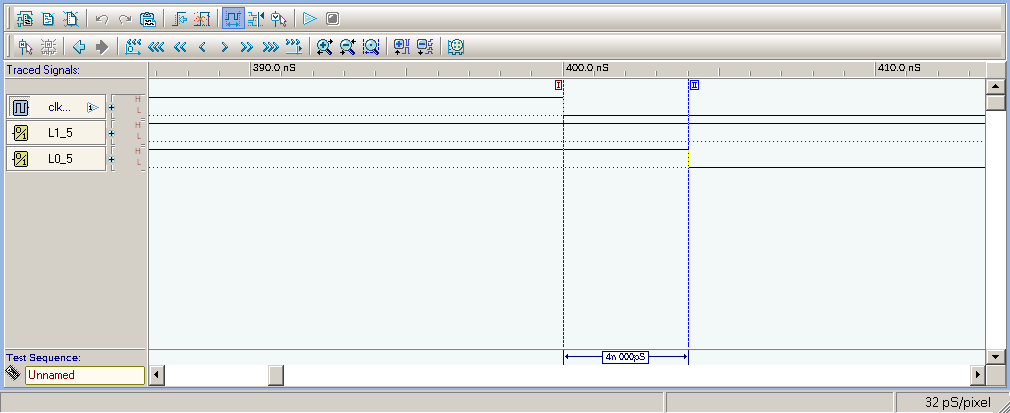
\includegraphics[width=.9\textwidth]{Exp04/exp4_2.0_d_clk_wave_lenght_ao_voltar_para_zero.png}
    \caption{Tamanho do pulso existente quando \textbf{A} retorna ao nível 0}\label{fig:exp4_2.0_d_clk_wave_lenght_ao_voltar_para_zero.png}
\end{figure}

\begin{enumerate}[E)]
\item \textbf{Haveria pulso em L0 caso houvesse um número par de portas NOT?}
\end{enumerate}

Sim poderia existir um pulso em \textbf{L0}. O único limitante para a observação
de pulsos é a quantidade de portas \textbf{NOT} existentes no circuito. O motivo
é o mesmo do item anterior: quanto maior o número de portas, maior será o delay
no circuito lógico; Caso o delay acarrete em uma superposição entre o nível
lógico de \textbf{A} e \textbf{L1}, então haverá um pulso em \textbf{L0}. Ou
seja, o pulso é apenas limitado à introdução de um delay suficientemente grande
no circuito.

Como prova dessa afirmação, é apresentado um circuito com número \emph{par} de
portas \textbf{NOT}, e que ainda assim possui pulsos em \textbf{L0}.

\begin{figure}[H]
    \centering
    \includegraphics[width=.9\textwidth]{Exp04/exp4_2.0_e_clk_circuito.png}
    \caption{Circuito com pulso em \textbf{L0} usando número \emph{par} de portas \textbf{NOT}}\label{fig:exp4_2.0_e_clk_circuito.png}
\end{figure}

\begin{figure}[H]
    \centering
    \includegraphics[width=.9\textwidth]{Exp04/exp4_2.0_e_clk_circuito_wave.png}
    \caption{Formato de onda do circuito com pulso}\label{fig:exp4_2.0_e_clk_circuito_wave.png}
\end{figure}


\subsection{Comparador de palavras de \(3\) \emph{bits}}\label{sec:comparador_de_palavras_3_bits}

\begin{enumerate}[A)]
\item \textbf{Completando a tabela verdade para um circuito \textbf{XNOR}}
\end{enumerate}

Para fazermos a tabela verdade do circuito proposto no enunciado, basta notarmos
a própria definição de uma porta \textbf{XNOR}; Sendo assim, teremos:

\begin{table}[H]
    \centering
    \caption{Tabela Verdade para o circuito \textbf{XNOR}}
    \begin{tabular}{|c|c|c|c|c|}\hline
    \multicolumn{2}{|c|}{Entradas} & \multicolumn{1}{|c|}{Saída} \\\hline
    $A_{i}$ & $B_{i}$ & $Z_{i}$ \\\hline
    0 & 0 & 1 \\\hline
    0 & 1 & 0 \\\hline
    1 & 0 & 0 \\\hline
    1 & 1 & 1 \\\hline
    \end{tabular}\label{tab:comparador_de_palavras_3_bits}
\end{table}

\begin{enumerate}[B)]
\item \textbf{Implementação da função lógica $Z_{i}$ apenas com portas NAND}
\end{enumerate}

Para implementarmos um circuito lógico \textbf{XNOR} usando apenas portas
\textbf{NAND}, podemos usar o circuito a seguir:

\begin{equation}
\overline{\left( \overline{(\overline{A_{i} \cdot A_{i}}) \cdot (\overline{B_{i} \cdot B_{i}})} \right) \cdot (\overline{A_{i} \cdot B_{i}})}
\end{equation}

\begin{enumerate}[C)]
\item \textbf{TODO}
\end{enumerate}

\begin{enumerate}[D)]
\item \textbf{Circuito comparador de palavras de 3 bits}
\end{enumerate}

Para montarmos o circuito total pedido no enunciado, basta usarmos $3$ dos
blocos implementados no item anterior, fazendo um \textbf{AND} entre cada uma
das $3$ saídas. Caso cada um dos blocos retorne o nível lógico $1$, então
teremos que o output final também será com nível lógico $1$, e, caso contrário,
o nível $0$. Existe, entretanto, um requisito: devemos montar esse circuito
apenas com portas \textbf{NAND} de $2$ entradas; Sendo assim, apresentamos um
circuito que satisfaz os requisitos necessários para o objetivo desejado:

\begin{figure}[H]
    \centering
    \includegraphics[width=.9\textwidth]{Exp04/exp4_2.1_d_circuito.png}
    \caption{Circuito Comparador de palavras de 3 bits}\label{fig:exp4_2.1_d_circuito.png}
\end{figure}

Reproduzimos a seguir a tabela verdade do circuito final. Contudo, Faz-se
necessário uma ressalva: como o circuito final possui $6$ valores de input, isso
acarreta em uma tabela com $2^{6} = 64$ linhas. Uma tabela assim seria muito
grande para reproduzirmos aqui. Dessa forma, optamos por somente mostrar os
inputs que produzem um output com valor igual a $1$. Todas as demais combinações
são assumidas como produzindo o output de nível lógico $0$.

\begin{table}[H]
    \centering
    \caption{Tabela Verdade para o circuito geral}
    \begin{tabular}{|c|c|c|c|c|c|c|}\hline
    \multicolumn{6}{|c|}{Entradas} & \multicolumn{1}{|c|}{Saída} \\\hline
    $A_{1}$ & $A_{2}$ & $A_{3}$ & $B_{1}$ & $B_{2}$ & $B_{3}$ & $Z_{i}$ \\\hline
    0 & 0 & 0 & 0 & 0 & 0 & 1 \\\hline
    0 & 0 & 1 & 0 & 0 & 1 & 1 \\\hline
    0 & 1 & 0 & 0 & 1 & 0 & 1 \\\hline
    0 & 1 & 1 & 0 & 1 & 1 & 1 \\\hline
    1 & 0 & 0 & 1 & 0 & 0 & 1 \\\hline
    1 & 0 & 1 & 1 & 0 & 1 & 1 \\\hline
    1 & 1 & 0 & 1 & 1 & 0 & 1 \\\hline
    1 & 1 & 1 & 1 & 1 & 1 & 1 \\\hline
    \end{tabular}\label{tab:comparador_de_palavras_3_bits}
\end{table}


\begin{enumerate}[E)]
\item \textbf{Circuito comparador de palavras de 3 bits}
\end{enumerate}

\section{Análise dos Resultados}
\label{sec:Resultados}

TODO

\section{Conclusão}
\label{sec:Conclusao}

TODO

\nocite{*}
\bibliographystyle{sbc}
\bibliography{relatorio}  %Aqui é a definição do arquivo .bib a ser usado pelas referências


\newpage
% Colocar aqui apenas as respostas dos itens da Auto-Avaliação
\section*{Auto-Avaliação}

Respostas:

TODO
% \begin{table}[H]
%     \begin{tabular}{|c|c|} \hline
%     \textbf{A} & \textbf{B}\\
%     \hline
%     1 & b \\ \hline
%     2 & d \\ \hline
%     3 & c \\ \hline
%     4 & a \\ \hline
%     5 & d \\ \hline
%     \end{tabular}
% \end{table}


\end{document}
